\chapter{The Best Financial Decision That Was Not Quite Theirs}

This chapter follows a short School of Hard Knocks entrepreneurship interview curated by LazyingArt LLC for Video2Book. The question is simple: what was the best financial decision you ever made? The answer begins with self-investment, then turns into a more interesting business episode: a profitable, fast-growing company sought venture capital, spent energy courting it, was passed over, and later saw that rejection as a fortunate outcome. There is no blackboard mathematics in the source, so the equations below are a compact decision language for the business mechanism reported in the transcript.

\section{The Question}

The opening question is direct: what was the best financial decision ever made? The first answer is also direct: investing in oneself. That answer matters because it sets the scale of the problem. A financial decision is not only a transaction; it can be an allocation of time, skill, judgment, and attention.

But the speaker does not stop with the slogan. He moves immediately from the personal answer to the founding period of a company. The shift is important. We are no longer asking whether self-investment is good in the abstract. We are asking how founders decide when a growing company should trade some independence and attention for outside capital.

Let us name the initial condition in the most cautious way possible:
\begin{equation}
\Pi > 0 .
\end{equation}
Here \(\Pi\) simply records the transcript's claim that the company was profitable. It is not a measured profit margin, a valuation, or a complete financial statement.

\section{A Profitable Company Looking For Speed}

The company was already growing quickly and was already profitable. That is the first constraint on the story. The founders were not describing an emergency financing round. They believed that additional capital could help them expand faster.

In symbols, the stated motive was not
\begin{equation}
K_{\mathrm{outside}} \rightarrow \text{survival},
\end{equation}
but rather
\begin{equation}
K_{\mathrm{outside}} \rightarrow \text{faster expansion}.
\end{equation}
That difference changes the whole interpretation. If capital is needed for survival, the decision is constrained by necessity. If capital is wanted for speed, the founders must compare the gain in speed against the costs of obtaining and accepting the money.

\begin{definition}
In this chapter, \(K_{\mathrm{outside}}\) denotes outside capital, specifically venture capital in the interview. \(A_{\mathrm{growth}}\) denotes the expected acceleration from that capital, while \(C_{\mathrm{attention}}\) denotes the time, energy, and focus consumed by the fundraising process.
\end{definition}

The transcript supports \(A_{\mathrm{growth}}\) and \(C_{\mathrm{attention}}\) directly: the founders wanted to expand faster, and the process took energy and attention. Other costs, such as dilution or control, are common entrepreneurial considerations, but they are not stated in this short excerpt and must be handled cautiously.

\section{The Venture Capital Courtship}

The founders sought out a venture capital firm. The word that carries the rhythm of the story is ``courtship.'' A courtship is not a single meeting. It is repeated attention: explanation, persuasion, follow-up, adjustment, waiting, and emotional energy.

A compact reconstruction of the decision looks like this:
\begin{equation}
V_{\mathrm{net}}
\approx
A_{\mathrm{growth}}
-
C_{\mathrm{attention}}
-
C_{\mathrm{control}}
-
C_{\mathrm{dilution}} .
\end{equation}
Only part of this expression is transcript-backed. The acceleration term is the reason they sought money. The attention term is the cost the speaker emphasizes. The control and dilution terms are standard additions to the outside-capital decision, not facts reported in the interview.

For this particular story, the central inequality is therefore narrower:
\begin{equation}
A_{\mathrm{growth}} \quad \hbox{must justify} \quad C_{\mathrm{attention}} .
\end{equation}
Before any term sheet is signed, the process itself can already consume founder capacity.

\begin{figure}
\centering
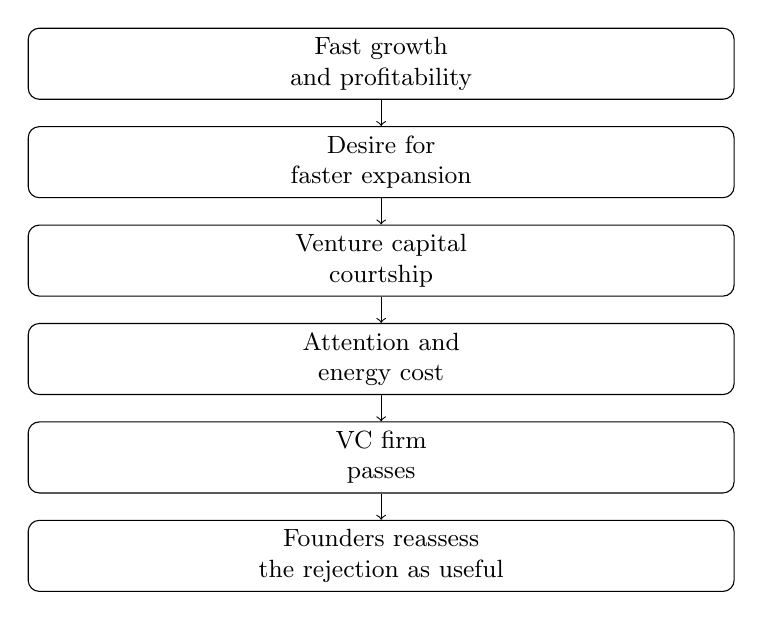
\begin{tikzpicture}[x=1cm,y=1cm, font=\small]
\node[draw, rounded corners, align=center, text width=.72\linewidth, minimum height=.75cm] (a) at (0,0) {Fast growth\\and profitability};
\node[draw, rounded corners, align=center, text width=.72\linewidth, minimum height=.75cm] (b) at (0,-1.25) {Desire for\\faster expansion};
\node[draw, rounded corners, align=center, text width=.72\linewidth, minimum height=.75cm] (c) at (0,-2.50) {Venture capital\\courtship};
\node[draw, rounded corners, align=center, text width=.72\linewidth, minimum height=.75cm] (d) at (0,-3.75) {Attention and\\energy cost};
\node[draw, rounded corners, align=center, text width=.72\linewidth, minimum height=.75cm] (e) at (0,-5.00) {VC firm\\passes};
\node[draw, rounded corners, align=center, text width=.72\linewidth, minimum height=.75cm] (f) at (0,-6.25) {Founders reassess\\the rejection as useful};
\draw[->] (a) -- (b);
\draw[->] (b) -- (c);
\draw[->] (c) -- (d);
\draw[->] (d) -- (e);
\draw[->] (e) -- (f);
\end{tikzpicture}
\caption{A transcript-backed reconstruction of the local decision sequence: profitable growth led to a search for speed, but the fundraising process exposed a cost in attention.}
\end{figure}

\subsection{Question \& Answer}

\paragraph{Question.}
If venture capital was supposed to help the company grow faster, why did the founders later feel glad when the firm passed?

\paragraph{Answer.}
Because the process revealed a hidden cost. The founders were not merely evaluating money. They were spending attention. The attempted raise became a live demonstration that outside capital can demand founder energy before it delivers any benefit.

The decision can be written as a simple test:
\begin{equation}
\text{Seek outside capital only if } V_{\mathrm{net}} > 0 .
\end{equation}
In this case, the rejection prevented the founders from continuing down a process they already found frustrating. The pass was made by the investor, but the interpretation belonged to the founders. They could recognize that the company still had growth, profit, and focus.

\section{A Worked Decision Example}

The transcript gives no numbers, so the following is not a reconstruction of the company's actual finances. It is a small worked example showing how the logic of the interview can be made explicit.

Suppose a founder estimates the benefit of outside capital as an acceleration value \(A_{\mathrm{growth}}\). Against that, we subtract the costs that matter to the decision:
\begin{align}
V_{\mathrm{net}}
&=
A_{\mathrm{growth}}
-
C_{\mathrm{attention}}
-
C_{\mathrm{control}}
-
C_{\mathrm{dilution}} .
\end{align}
Now consider the narrow version supported most directly by the interview. Let the founder initially ignore control and dilution because no deal has been reached yet:
\begin{align}
V_{\mathrm{process}}
&=
A_{\mathrm{growth}}
-
C_{\mathrm{attention}} .
\end{align}
The fundraising process is worth continuing only if
\begin{align}
A_{\mathrm{growth}} &> C_{\mathrm{attention}} .
\end{align}
If the courtship keeps consuming energy while the probability of a deal falls, then the expected acceleration shrinks. A more explicit process version is
\begin{align}
V_{\mathrm{process}}
&=
p_{\mathrm{deal}} A_{\mathrm{growth}}
-
C_{\mathrm{attention}},
\end{align}
where \(p_{\mathrm{deal}}\) is the founders' estimated probability that the fundraising process will actually produce useful capital.

As the courtship drags on, two things can happen at once:
\begin{align}
p_{\mathrm{deal}} &\downarrow,\\
C_{\mathrm{attention}} &\uparrow.
\end{align}
Then \(V_{\mathrm{process}}\) can become negative even before any ownership dilution is considered. That is the mechanism behind the interview's reversal: the founders wanted capital, but the process made the cost visible.

\section{The Decision That Was Not Fully Theirs}

The speaker says the best decision was not really their decision, but it kind of was. That sentence carries the paradox. The venture capital firm made the formal decision to pass. The founders did not choose the rejection in the moment.

But they did choose to seek the capital, to endure the courtship for a time, and then to understand the result. Entrepreneurship often works this way. Not every outcome is chosen, but outcomes still have to be interpreted. The skill is not only deciding in advance. It is also recognizing when an external no has preserved something valuable.

\begin{remark}
The lesson is not that venture capital is bad. The transcript does not support that broad claim. The supported claim is narrower and more useful: capital has process costs, and those costs can matter even when the company is already growing.
\end{remark}

\section{Summary}

The chapter's movement is from a simple answer to a more precise business judgment. The best financial decision begins as self-investment, then becomes a story about a profitable company that wanted capital to grow faster. The founders entered a venture capital courtship, spent energy on it, and were passed over. In hindsight, the pass looked beneficial because the process itself had revealed the price of outside capital in attention and frustration.

The durable principle is cautious: outside money should be judged not only by the cash it brings, but by the attention it consumes and the independence it may alter. In this interview, the important object was not merely \(K_{\mathrm{outside}}\). It was the net value after the hidden costs were counted.